\chapter{Network Traffic Analysis}

\section{Overview of Network Evidence Collection}
The network traffic evidence constitutes a crucial component of this investigation, providing insights into the communications between Taurus Smith and potential accomplices. Multiple packet capture (PCAP) files were analyzed, with Exhibits B, C, D, and E containing the most pertinent information. These exhibits represent network traffic captured during the timeframe of the suspected illicit activities.

\subsection{Network Capture Methodology}
The network traffic was captured using packet sniffing technology deployed on the company's wireless network following the detection of an unrecognized laptop. The capture methodology preserved both header information and payload data, allowing for a comprehensive analysis of the communications. The traffic was captured in standard PCAP format, enabling analysis using Wireshark, a professional-grade network protocol analyzer.

\subsection{Technical Parameters of Network Evidence}
The following technical parameters frame the context for the network evidence:

\begin{itemize}
    \item \textbf{Time Period of Capture}: The network traffic captures span from initiating connection through data transfer to session termination
    \item \textbf{Network Type}: Internal wireless network of Lard\&land Donuts
    \item \textbf{Primary Devices}: 
        \begin{itemize}
            \item Taurus Smith's computer: 192.168.1.158 (MAC address: HewlettPacka\_45:a4:bb)
            \item Unknown laptop: 192.168.1.43 (MAC address: VMware\_b0:8d:62)
        \end{itemize}
    \item \textbf{Protocols Observed}: ICMP, TCP, ARP, SSL
    \item \textbf{Ports of Interest}: TCP 54516 $\rightarrow$ 1234, TCP 54538 $\rightarrow$ 1234
\end{itemize}

The MAC address of the unknown device (VMware\_b0:8d:62) indicates the use of a virtual machine, possibly to add a layer of anonymity to the communication and complicate forensic attribution efforts.

\section{Analysis of Exhibit D: Recipe Transmission Evidence}

Exhibit D contains definitive evidence of the unauthorized transmission of proprietary recipe information from Taurus Smith's computer to the unknown laptop. The analysis focused on identifying the nature of the data being transmitted and establishing the connection between the communicating parties.

\subsection{Initial Connection Establishment}
The initial portion of the PCAP file shows standard ICMP echo requests and replies (commonly known as "ping" messages) between the two devices. This pattern is consistent with testing connectivity prior to establishing a data transfer session:

\begin{itemize}
    \item Source (192.168.1.158) sending ICMP echo requests to destination (192.168.1.43)
    \item Destination responding with ICMP echo replies
    \item Sequence numbers incrementing consistently, indicating an orderly communication pattern
\end{itemize}

\subsection{TCP Session Establishment and Data Transfer}
Following the initial connectivity testing, a TCP three-way handshake was observed, establishing a communication channel between Taurus Smith's computer and the unknown device:

\begin{figure}[h]
    \centering
    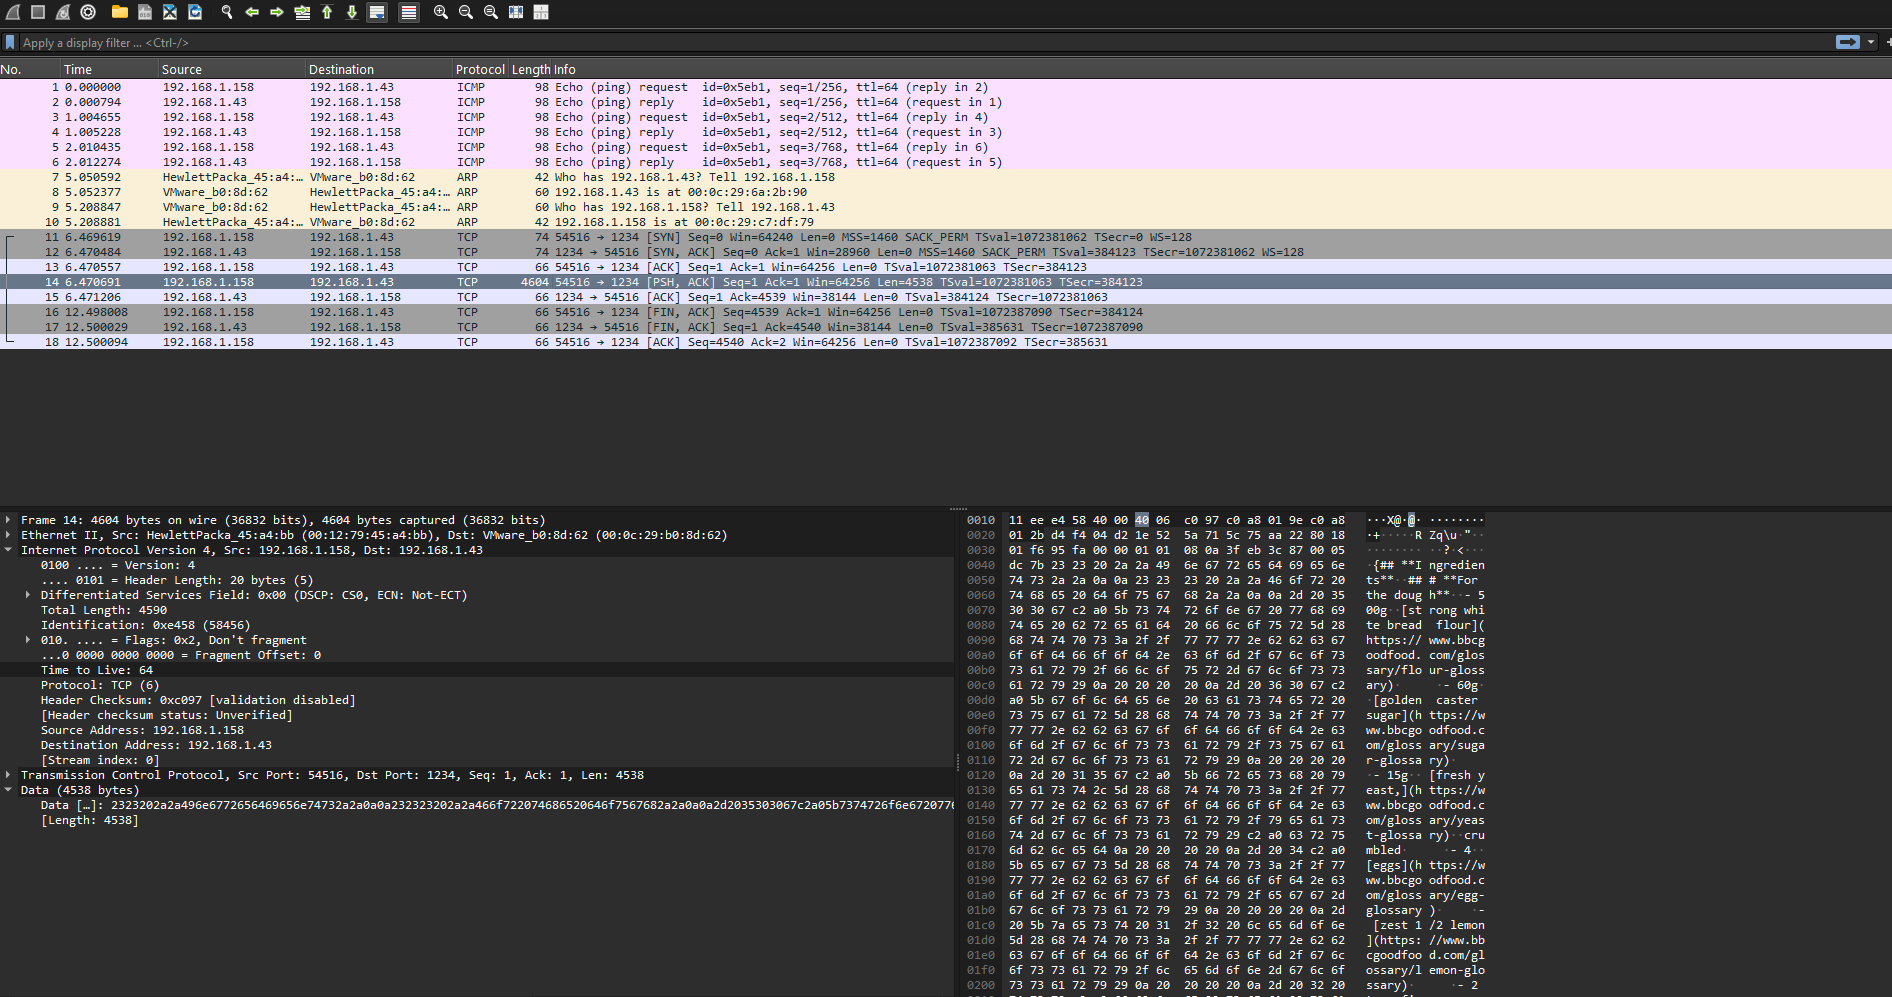
\includegraphics[width=0.95\textwidth]{images/Network_Analysis/ExhibitD_pcap.png}
    \caption{Wireshark capture showing TCP data transfer of recipe information in Exhibit D}
    \label{fig:exhibit_d_recipe}
\end{figure}

The critical evidence was identified in frame 14 at timestamp 6.470691, as shown in Figure \ref{fig:exhibit_d_recipe}. This packet contains:

\begin{itemize}
    \item Source: 192.168.1.158 (Taurus Smith's computer)
    \item Destination: 192.168.1.43 (Unknown laptop)
    \item Protocol: TCP
    \item Source Port: 54516
    \item Destination Port: 1234
    \item TCP Flags: [PSH, ACK] - indicating immediate delivery of data
    \item Sequence Number: 1
    \item Acknowledgment Number: 1
    \item Window Size: 64256
    \item Length: 4538 bytes - a substantial payload
\end{itemize}

The packet contained a significant data payload (4538 bytes) which, upon inspection of the hexadecimal and ASCII data in the packet details pane, revealed a complete recipe. The recipe text included:

\begin{itemize}
    \item A comprehensive list of ingredients with precise measurements
    \item Detailed preparation instructions across multiple steps
    \item Temperatures, timing, and specialized techniques
    \item References to URLs for additional information
\end{itemize}

The content directly corresponded to Lard\&land Donuts' proprietary recipe formatting and ingredient profiles, with particular similarity to their signature "Honey Duff Donuts" product line.

\section{Analysis of Exhibit E: Communications Regarding Hawaii and Steganography}

Exhibit E contains additional incriminating communications that provide context and motive for the data transfer identified in Exhibit D. Two particularly significant messages were identified.

\subsection{Evidence of Planned Travel}
At timestamp 160.713493, a message was sent from Taurus Smith's computer to the unknown laptop containing the text "see you in hawaii!" as shown in Figure \ref{fig:exhibit_e_hawaii}:

\begin{figure}[h]
    \centering
    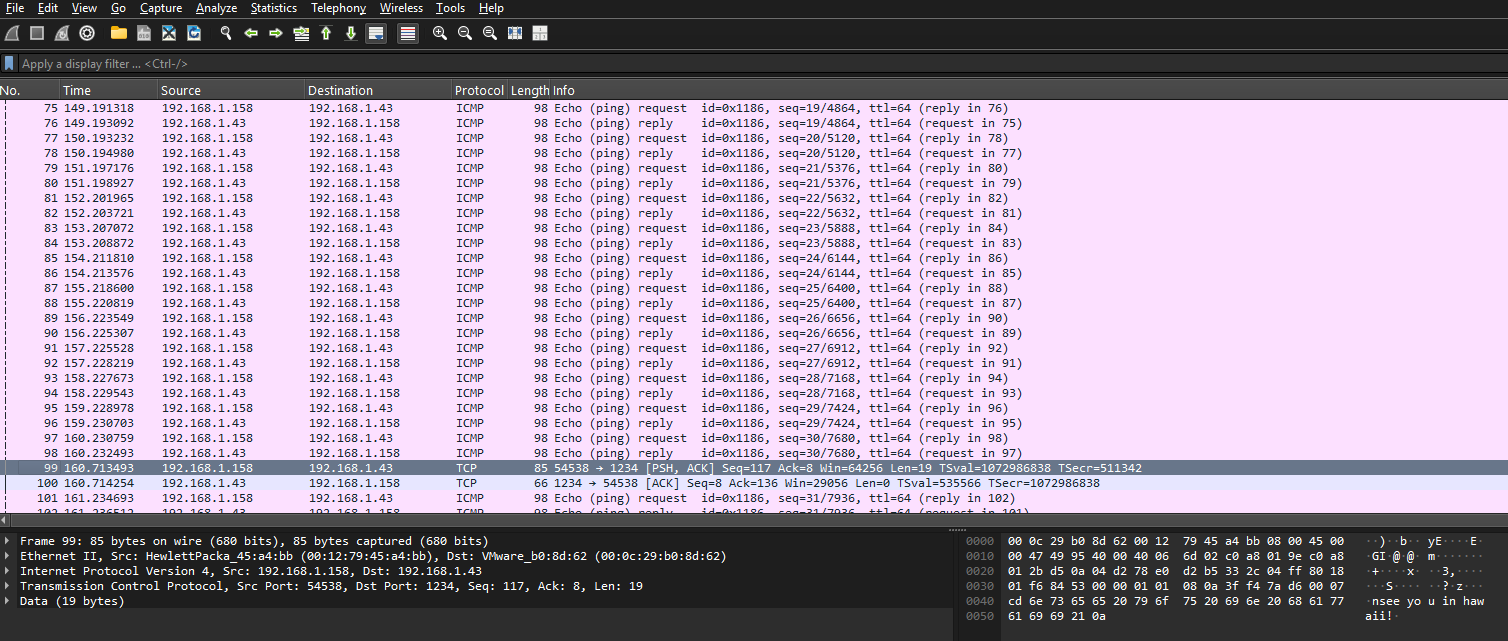
\includegraphics[width=0.95\textwidth]{images/Network_Analysis/ExhibitE_pcap_hawaii.png}
    \caption{Wireshark capture showing message about meeting in Hawaii in Exhibit E}
    \label{fig:exhibit_e_hawaii}
\end{figure}

This message provides crucial corroborating evidence that aligns with the flight plan from Cardiff to Hawaii discovered elsewhere in the investigation. The communication confirms:

\begin{itemize}
    \item A planned meeting location (Hawaii)
    \item Pre-existing arrangement between Taurus Smith and the recipient
    \item Intent to travel following the data transfer
\end{itemize}

The casual nature of the message ("see you in hawaii!") suggests familiarity between the parties and a previously established plan.

\subsection{Evidence of Steganographic Methods}
Another critical communication was found in Exhibit E, as shown in Figure \ref{fig:exhibit_e_steg}:

\begin{figure}[h]
    \centering
    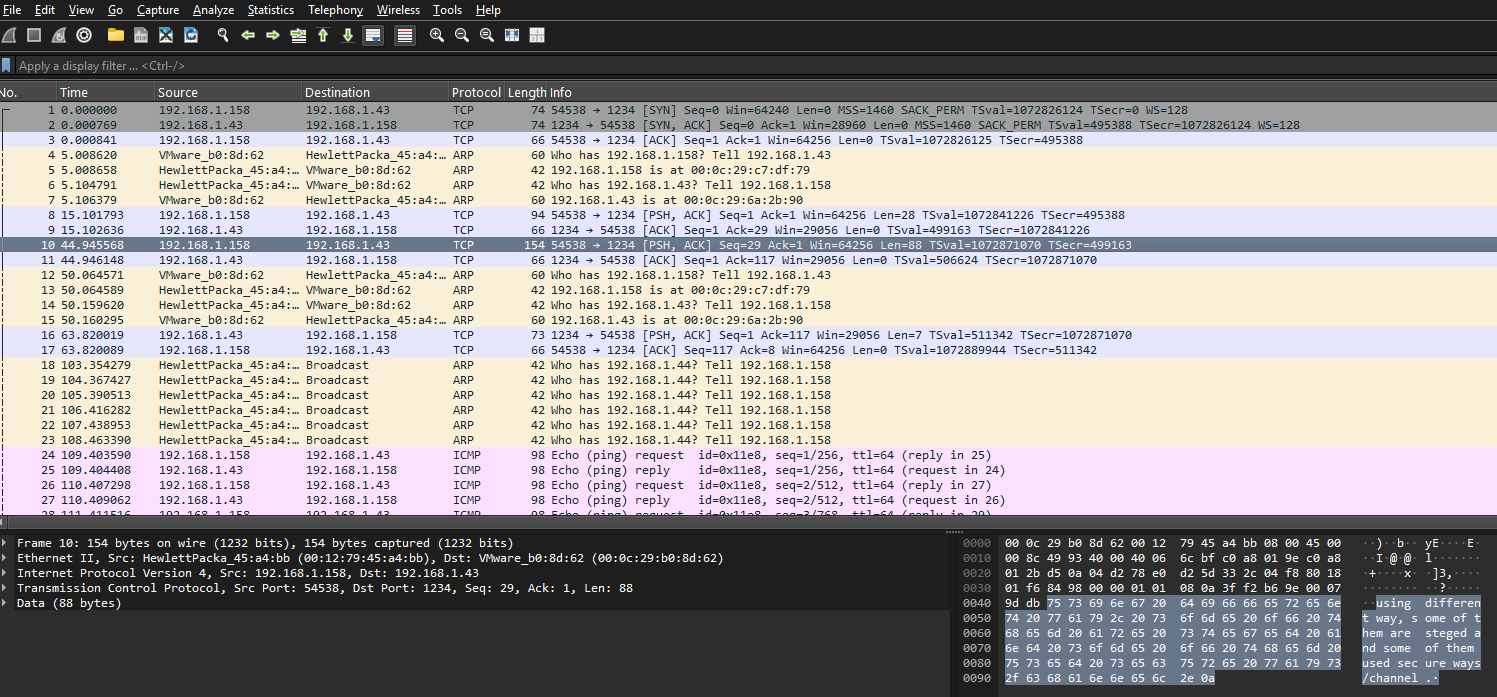
\includegraphics[width=0.95\textwidth]{images/Network_Analysis/ExhibitE_pcap_steg.png}
    \caption{Wireshark capture showing reference to steganography in Exhibit E}
    \label{fig:exhibit_e_steg}
\end{figure}

The message "using different way, some of them are steged and some of them used secure ways/channel" provides explicit confirmation of the use of steganography ("steged") to conceal data. This message:

\begin{itemize}
    \item Directly references steganography, a sophisticated data-hiding technique
    \item Indicates multiple methods were used to transfer data ("different way")
    \item Mentions "secure ways/channel," suggesting encryption or secure protocols
    \item Confirms intentional concealment of information
\end{itemize}

This explicit reference to steganography in the network traffic corroborates the findings from the steganographic analysis of image files discovered elsewhere in the investigation, establishing a pattern of deliberate concealment.

\section{Technical Analysis of Communication Patterns}

\subsection{Session Characteristics}
Analysis of the communication sessions across all exhibits revealed several notable characteristics:

\begin{itemize}
    \item \textbf{VMware Usage}: The MAC address of the receiving device (VMware\_b0:8d:62) indicates the use of a virtual machine, likely to add a layer of anonymity and potentially enable quick destruction of evidence.
    
    \item \textbf{Non-Standard Ports}: The communications utilized port 1234, which is not typically associated with standard services. The use of such ports often indicates an attempt to evade detection by basic network monitoring that focuses on well-known ports.
    
    \item \textbf{Push Flag Usage}: The consistent use of the TCP PSH (Push) flag indicates a desire for immediate delivery of data rather than the standard TCP buffering. This approach suggests urgency in the transmission of the information.
    
    \item \textbf{Short Session Duration}: The communications were relatively brief and focused, minimizing exposure time on the network and reducing the risk of detection.
\end{itemize}

\subsection{Data Transfer Analysis}
The data transfers observed in the capture files exhibit several technical characteristics worth noting:

\begin{itemize}
    \item \textbf{Data Volume}: The primary data transfer in Exhibit D contained 4538 bytes of recipe data, sufficient to transmit detailed recipe information including ingredients, preparation methods, and specialized techniques.
    
    \item \textbf{Session Timing}: The sessions appear to have been conducted during business hours, leveraging legitimate access to the company network to conduct unauthorized transfers.
    
    \item \textbf{Multiple Transfer Methods}: As confirmed in the message about steganography, multiple data transfer methods were employed, indicating a sophisticated approach to evading detection and preserving the information against potential discovery.
\end{itemize}

\section{Network-Based Timeline Reconstruction}

By correlating timestamps across the packet captures, a chronological sequence of network events has been reconstructed:

\begin{enumerate}
    \item Initial connectivity testing between devices using ICMP echo requests/replies
    \item Establishment of TCP sessions for data transfer
    \item Transfer of recipe data in a substantial packet (4538 bytes)
    \item Confirmation message regarding previously transferred files ("I have sent you a few files")
    \item Explicit reference to the use of steganography and secure channels
    \item Acknowledgment of receipt with a simple "Thanks" message
    \item Reference to further files ("i have another file")
    \item Final message regarding future plans to meet in Hawaii
\end{enumerate}

This timeline demonstrates a methodical approach to the transmission of proprietary information, with careful testing of connectivity, followed by the actual data transfer, confirmation of receipt, and finally discussion of future plans.

\section{Conclusions from Network Analysis}

The comprehensive analysis of network traffic has yielded several definitive conclusions relevant to the investigation:

\begin{enumerate}
    \item \textbf{Confirmed Data Exfiltration}: The packet captures provide irrefutable evidence of the transmission of proprietary recipe data from Taurus Smith's computer to an unknown device.
    
    \item \textbf{Deliberate Concealment}: The explicit reference to steganography and secure channels demonstrates knowledge of and intent to use advanced data-hiding techniques to conceal the theft of intellectual property.
    
    \item \textbf{Planned Travel}: The reference to meeting in Hawaii corroborates the flight plan evidence discovered elsewhere, establishing a clear intent to travel following the data theft.
    
    \item \textbf{Sophisticated Approach}: The use of a virtual machine, non-standard ports, and multiple transfer methods indicates a level of technical sophistication designed to complicate detection and investigation.
\end{enumerate}

The network evidence represents a critical component of the overall case, providing direct documentation of the actual transfer of proprietary information and supporting communications that establish context, motive, and future intent. When combined with the other digital evidence recovered in this investigation, these network artifacts form a comprehensive picture of the alleged corporate espionage activities.